% Created 2023-08-08 Tue 22:03
% Intended LaTeX compiler: pdflatex
\documentclass[11pt]{article}
\input{page-size}
\input{generic}
\input{math}
\input{font-selection}
\author{Jihuan Tian}
\date{\today}
\title{The star of a subset of simplices}
\hypersetup{
 pdfauthor={Jihuan Tian},
 pdftitle={The star of a subset of simplices},
 pdfkeywords={},
 pdfsubject={},
 pdfcreator={Emacs 27.1 (Org mode 9.4)}, 
 pdflang={English}}
\begin{document}

\maketitle
\setcounter{tocdepth}{5}
\tableofcontents

In \href{https://www.youtube.com/playlist?list=PL9\_jI1bdZmz0hIrNCMQW1YmZysAiIYSSS}{CMU DDG course} \href{https://youtu.be/TDic3pJyYb8?list=PL9\_jI1bdZmz0hIrNCMQW1YmZysAiIYSSS\&t=2547}{Lecture 2A}, the star of a subset of simplices is defined as the union of \textbf{simplices} but \textbf{not simplicial complex} which contains the given subset of simplices. Therefore, for the central vertex \(v_1\) as shown below, all edges and cells in red color form its star. The edges and vertices on the boundary do not belong to the star, even though they belong to the simplicial complex formed by the cells with their lower dimensional descendants. Take cell 1 as example, the boundary edge \(\left\{ v_2, v_3 \right\}\) and the boundary vertices \(v_2\) and \(v_3\) are contained in the simplicial complex formed by cell 1 and its lower dimensional descendants, i.e. \(\left\{ \left\{ v_1,v_2,v_3 \right\}, \left\{ v_1,v_2 \right\}, \left\{ v_2,v_3 \right\}, \left\{ v_3,v_1 \right\}, \left\{ v_1 \right\}, \left\{ v_2 \right\}, \left\{ v_3 \right\}, \emptyset \right\}\). However, they are not contained in the cell 1 itself as a 2-simplex, i.e. \(\left\{ v_1,v_2,v_3 \right\}\).
\begin{center}
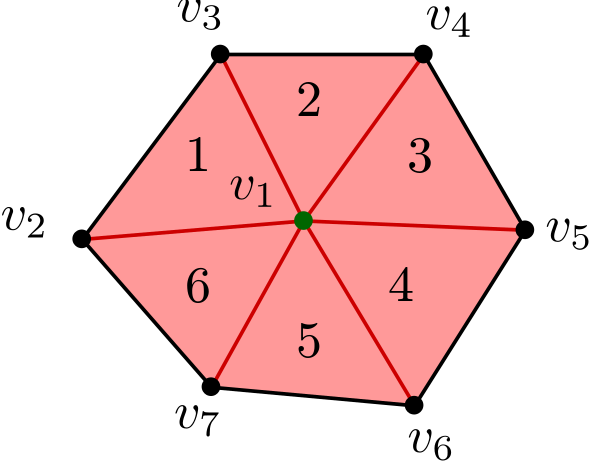
\includegraphics[width=0.5\textwidth]{figures/2023-07-03-star-of-simplices.png}
\end{center}
\href{../../../academic/math/docs/schematics/2023-07-03-star-of-simplices.odg}{Link to odg illustration}
\end{document}